\documentclass[conference]{IEEEtran}
\IEEEoverridecommandlockouts
% The preceding line is only needed to identify funding in the first footnote. If that is unneeded, please comment it out.
\usepackage{cite}
\usepackage{amsmath,amssymb,amsfonts}
\usepackage{algorithmic}
\usepackage{graphicx}
\usepackage{textcomp}
\usepackage{booktabs}
\usepackage{xcolor}
\def\BibTeX{{\rm B\kern-.05em{\sc i\kern-.025em b}\kern-.08em
    T\kern-.1667em\lower.7ex\hbox{E}\kern-.125emX}}
\begin{document}

\title{Multi-modal SAR Robot}
% {\footnotesize \textsuperscript{*}Note: Sub-titles are not captured in Xplore and
% should not be used}
% \thanks{Identify applicable funding agency here. If none, delete this.}
% }

\author{
    \IEEEauthorblockN{
        Bintang Dwi Marthen\IEEEauthorrefmark{1}\IEEEauthorrefmark{3},
        Kenneth Ezekiel Suprantoni\IEEEauthorrefmark{1}\IEEEauthorrefmark{3},
        Manuella Ivana Uli Sianipar\IEEEauthorrefmark{1}\IEEEauthorrefmark{3},
        Reza Pahlevi Ubaidillah\IEEEauthorrefmark{1}\IEEEauthorrefmark{3}, \\
        Priya Qolbu Dhiya'an Amar\IEEEauthorrefmark{1},
        Alghifari Mahfudz Rumi\IEEEauthorrefmark{2},
        Nana Sutisna\IEEEauthorrefmark{1},
        Infall Syafalni\IEEEauthorrefmark{1}, and
        Trio Adiono\IEEEauthorrefmark{1}
    }
    \IEEEauthorblockA{
        \IEEEauthorrefmark{1}School of Electrical Engineering and Informatics, 
        Institut Teknologi Bandung, Bandung, Indonesia \\
        \{marthen.bintangdwi, ken35kiel, manuellaivanauli, rezapuobed, priyaqda\}@gmail.com, \{nsutisna, infall, tadiono\}@itb.ac.id
    }
    \IEEEauthorblockA{
        \IEEEauthorrefmark{2}Faculty of Mechanical and Aerospace Engineering, 
        Institut Teknologi Bandung, Bandung, Indonesia \\
        alghifari.mahfudz@gmail.com
    }
    \thanks{\IEEEauthorrefmark{3}These authors contributed equally to this work.}
}

\maketitle

\begin{abstract}
This document is a model and instructions for \LaTeX.
This and the IEEEtran.cls file define the components of your paper [title, text, heads, etc.]. *CRITICAL: Do Not Use Symbols, Special Characters, Footnotes, 
or Math in Paper Title or Abstract.
\end{abstract}

\begin{IEEEkeywords}
component, formatting, style, styling, insert
\end{IEEEkeywords}

\section{Introduction}
An effective and rapid response in the aftermath of natural or man-made disasters is a critical factor in the saving of human lives. Robotics has emerged as a vital tool for Search and Rescue (SAR) operations, capable of entering environments that are too hazardous for human first responders \cite{SARRobot}. However, a significant challenge persists: the vast diversity of disaster scenarios. The unique conditions of a collapsed building, a flooded area, or rugged wilderness terrain demand different robotic capabilities for mobility and sensing. This makes a single, monolithic robot design inefficient and impractical, highlighting the need for adaptable and versatile platforms.

To overcome this limitation, this paper introduces a modular multi-modal SAR robot designed on a "building block" principle. The core idea is to enable the rapid assembly and reconfiguration of the robot using specialized modules to match the specific demands of a rescue mission. This approach enhances operational flexibility, allowing teams to deploy a robot tailored for optimal performance in any given environment, a concept that is becoming increasingly important in the field of field robotics \cite{ModularRobotic}.

For victim detection, our system moves beyond simple visual searches, which are often ineffective in cluttered debris. We integrate a lightweight, power-efficient voice recognition module to detect human sounds, such as cries for help. This is achieved using Tiny Machine Learning (TinyML), where a compact neural network runs directly on a low-power microcontroller \cite{TinyML}. This on-board processing allows the robot to react to audio cues in real-time without depending on a stable, high-bandwidth connection to a remote operator, which is often unavailable in disaster zones.

Once a potential victim's sound is detected, pinpointing their location is the next crucial step. As GPS signals are unreliable or completely absent inside buildings or under rubble, our robot utilizes a WiFi Received Signal Strength Indicator (RSSI) localization system. By deploying two or more low-cost ESP32 modules as fixed beacons in the operational area, the robot uses the relative signal strength from each beacon to perform centroid based localization \cite{WSNCentroid}. This paper presents the design of this modular system and details the experimental validation of the TinyML-based sound recognition and the WiFi RSSI localization subsystems.


\section{Related Works}

\subsection{Modularity in SAR Robots}
Modularity in SAR robotics has been explored extensively, offering benefits including adaptability to diverse terrains, robustness to failure, and cost-effective scalability. Modular self-reconfigurable systems -- composed of standardized building blocks with uniform docking and communication interfaces -- can dynamically alter their shape and capabilities in response to environmental demands. For instance, PolyBot \cite{PolyBot} demonstrates sequential reconfiguration from snake-like locomotion to legged configurations, enhancing mobility over rubble and uneven surfaces, a key requirement in urban rescue scenarios.

Similarly, self-reconfigurable modular robots have been proposed for generality and resilience, with reconfiguration allowing navigation in confined spaces and recovery from actuator failure. Such systems can eject or rearrange modules to continue operations even when components malfunction. These capabilities align well with SAR needs where mechanical damage or terrain variability is common. Comprehensive reviews in field robotics emphasize that modularity supports rapid adaptation to mission-specific requirements, with plug-and-play payloads enabling teams to swap in appropriate locomotion (e.g., wheels, tracks, legs) or sensor (e.g., thermal, gas) modules as needed \cite{ModularRobotic}.

Despite its promise, true deployment of self-reconfigurable systems in real-world SAR remains limited. Challenges include durable docking mechanisms, distributed control, and scalability to many modules. A 2002 survey \cite{wiredBots2002} noted that while modular robots offered versatility, practical issues such as module complexity and control reliability were significant obstacles \cite{}. Nonetheless, ongoing research -- such as morphogenetic and CPG-controlled modular designs \cite{CPGLocomotion} -- continues to push capabilities, targeting robustness and autonomy in SAR and field robotics applications.

\subsection{Acoustic-Based Victim Detection}
TODO: manuella

\subsection{Indoor Localization in GPS-Denied Environments}
TODO: obed \cite{WSNCentroid} ini sitasi ke paper yang dipake di ppt mu


\section{System Architecture}
The architecture of the proposed Search and Rescue robot is founded on the principle of mission-specific modularity. The primary objective of this design is to create a platform where both hardware and software can be adapted for different operational environments, such as collapsed buildings or open-field disaster sites, while maintaining reasonable costs. This approach allows a rescue team to augment a core robotic platform with specialized capabilities as needed.

Our methodology leverages a standard, commercially available robotic base—the Robotis TurtleBot—which provides robust and reliable locomotion. The TurtleBot chassis features a grid of pre-drilled mounting holes, which serves as the physical interface for our modular "building block" concept. New functional modules are physically attached to the chassis using a simple and direct screw-on system. Electronically, each module is wired directly to the main onboard processor, allowing for straightforward integration of custom components into the main system.

\subsection{Hardware Implementation}
The physical prototype is constructed upon a Robotis TurtleBot3 Burger, which serves as the core platform for locomotion and control. The primary onboard computer is a Raspberry Pi 4B with 4GB of RAM. The TurtleBot's Dynamixel servos are managed by a dedicated OpenCR board, which interfaces with the Raspberry Pi.

Our modular additions are integrated directly onto this base platform. The acoustic sensing capability is provided by a standard USB clip-on microphone. To enhance directed listening and improve the signal-to-noise ratio, the microphone is mounted at the focal point of a parabolic dish, which is attached to a servo motor for orientation control. For the localization task, the robot is equipped with a dedicated ESP32 microcontroller that functions as the onboard WiFi receiver and processor for RSSI measurements.

The localization infrastructure consists of three stationary beacons, each built from a standalone ESP32 module powered by AAA batteries. These beacons are positioned around the operational area to create the necessary reference grid. The complete hardware assembly is depicted in the CAD model shown in Fig.~\ref{fig:robotCAD}. To provide a clear overview, the key hardware components are summarized in Table~\ref{tab:hardware_components}.

\begin{figure}[!b]
  \centering
  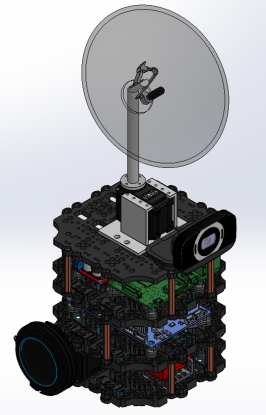
\includegraphics[width=0.65\linewidth]{img/robotcad.png}
  \caption{CAD model of the assembled SAR robot, showing the TurtleBot3 Burger base, onboard electronics, and sensor attachments}
  \label{fig:robotCAD}
\end{figure}

\begin{table*}[t]
  \caption{Key Hardware Components}
  \label{tab:hardware_components}
  \centering
  \begin{tabular}{lll}
    \toprule
    \textbf{Component} & \textbf{Model/Part} & \textbf{Purpose} \\
    \midrule
    Core Platform & Robotis TurtleBot3 Burger & Mobility and base structure \\
    Central Processor & Raspberry Pi 4B (4GB) & Main control, audio processing \\
    Low-level Control & OpenCR Board & Interfacing with Dynamixel servos \\
    Onboard RSSI RX & ESP32 & Dedicated WiFi RSSI processing \\
    Microphone & USB Clip-on Microphone with Parabolic Dish & Capturing ambient audio \\
    Localization Beacons & ESP32 (x3) & Stationary WiFi signal sources \\
    Power Source & TurtleBot3 Battery Pack & System power \\
    \bottomrule
  \end{tabular}
\end{table*}

\begin{figure}[!b]
  \centering
  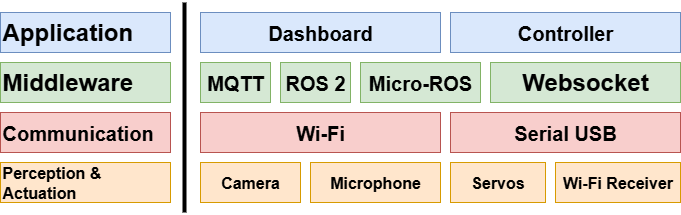
\includegraphics[width=0.65\linewidth]{img/layer.png}
  \caption{The layered IoT architecture of the system, showing the hierarchy from high-level application interfaces down to the physical perception and actuation components}
  \label{fig:layering}
\end{figure}

\subsection{Software and Data Flow}
The robot's architecture is organized into a four-tiered IoT stack, as illustrated in Fig.~\ref{fig:layering}. This layered approach separates high-level applications from the underlying hardware, promoting modularity. The stack consists of: the Application layer (user-facing dashboard and controller), the Middleware layer (handling data exchange via MQTT, Robot Operating System (ROS) 2, Micro-ROS, and WebSockets), the Communication layer (Wi-Fi and Serial USB), and the Perception \& Actuation Layer (physical sensors and actuators).

\begin{figure*}[!htbp]
  \centering
  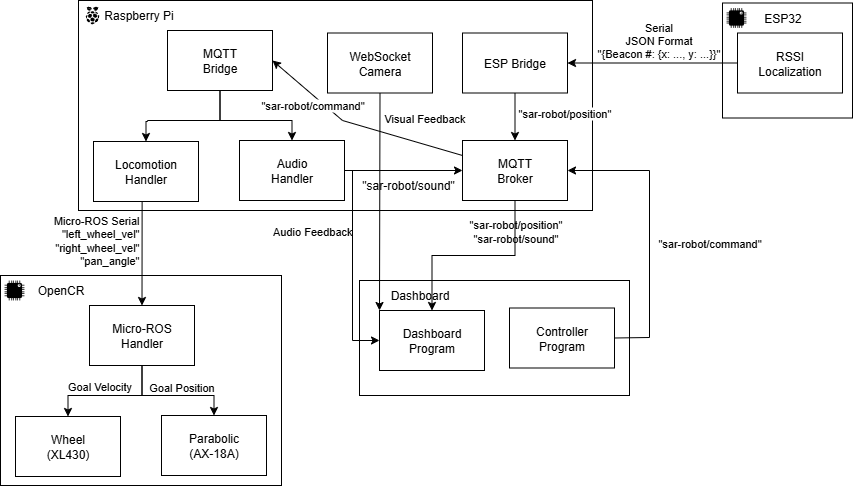
\includegraphics[width=0.65\textwidth]{img/DFD.png}
  \caption{A detailed block diagram of the software components and data flow. The MQTT Broker on the Raspberry Pi acts as a central hub, routing data such as commands, position, and sound detection between the various hardware and software modules.}
  \label{fig:dfd}
\end{figure*}

The operational data flow between the primary software modules is managed using a hybrid approach that combines custom Python scripts, the MQTT protocol for lightweight messaging, and elements of the ROS for hardware interfacing. The specific interactions are detailed in Fig.~\ref{fig:dfd}. The audio classification task on the Raspberry Pi is implemented using the TensorFlow library.

The operational flow of the system is continuous and concurrent:
\begin{enumerate}
    \item \textbf{Acoustic Perception:} The main Python script on the Raspberry Pi continuously listens for audio captured by the parabolic microphone. It processes this audio stream in real-time using a TensorFlow model trained to recognize human voice patterns. The system constantly publishes the results—including the sound's orientation relative to the robot and a confidence level of human presence—to an MQTT topic.
    \item \textbf{Localization:} Concurrently, the dedicated onboard ESP32 continuously scans for WiFi signals from the three stationary beacons. Each beacon is configured to broadcast a unique and constant WiFi network name (SSID). The onboard ESP32 measures the RSSI from each beacon and uses a pre-calibrated model based on a least-squares mapping to calculate the robot's (x, y) coordinates relative to the known positions of the beacons.
    \item \textbf{Data Aggregation and Transmission:} The Raspberry Pi subscribes to the data streams from both the acoustic perception script and the ESP32 localization module. It aggregates this information—the robot's current location and the confidence/direction of any detected human voice—and transmits it to a remote operator's computer for monitoring and decision-making.
\end{enumerate}


\section{Methodology}

\subsection{Human Voice Detection Model Preparation}
This study focuses on developing a lightweight acoustic model capable of distinguishing between human and non-human sounds for search-and-rescue (SAR) robotics. The model is optimized for deployment on edge devices using TinyML frameworks. The training pipeline involves dataset preparation, feature extraction, data augmentation, and supervised learning.

\subsubsection{Dataset Collection and Labeling}
We utilized a subset of the publicly available CHiME-Home dataset~\cite{Foster2015chime}, which contains domestic environmental audio recordings annotated with sound event labels. Audio segments featuring human vocal activity such as speech, calling, or shouting were manually extracted and labeled as “human,” while other segments (e.g., background noise, domestic appliances, animals) were labeled as “non-human.” The dataset was further balanced and curated to ensure consistent segment lengths of three seconds at a sampling rate of 16\,kHz.

\subsubsection{Spectrogram Feature Extraction}
To convert the audio signals into a format suitable for convolutional neural networks (CNNs), we applied mel-spectrogram transformation. Each audio clip was transformed into a 64-bin mel-spectrogram using a short-time Fourier transform (STFT) with parameters tuned for low-latency environments. The resulting spectrograms were normalized to a \([0, 1]\) range after applying logarithmic scaling and clipping to \([-80, 0]\) dB.

\subsubsection{Data Augmentation}
To improve generalization and robustness in noisy or reverberant environments, two augmentation strategies were employed:

\begin{itemize}
  \item \textbf{Additive Gaussian Noise:} Small random noise was added to spectrograms to simulate environmental interference.
  \item \textbf{Time Masking:} Inspired by SpecAugment~\cite{Park2019specaugment}, random temporal sections of spectrograms were zeroed out to simulate partial occlusion of acoustic features.
\end{itemize}

Each original spectrogram generated two augmented variants, tripling the effective dataset size.

\subsubsection{Model Training and Evaluation}
The dataset was split using stratified sampling into training and testing subsets (80\% / 20\%). The model architecture consisted of a compact 2D convolutional neural network designed to fit within the memory constraints of embedded hardware. The input shape was fixed at $64 \times 64 \times 1$. The model was trained using binary cross-entropy loss and Adam optimizer, with early stopping and learning rate reduction callbacks to prevent overfitting.

Evaluation was performed on the held-out test set using standard classification metrics including accuracy, precision, recall, F1-score, and confusion matrix. The final model achieved a test accuracy of 97.79\%, demonstrating strong generalization performance in distinguishing human from non-human sounds.

\subsection{Weighted Centroid Localization}
We collected RSSI measurements in an indoor corridor (Labtek 1 Mekanika Tanah, ITB) using three fixed ESP32 beacons and one mobile ESP32 receiver. Measurements were taken at five known distances (1.60m, 2.40m, 3.20m, 4.00m, 4.80m) yielding a total of 1574 samples. Each sample consists of the RSSI value from a beacon at a given distance. These raw RSSI values were then preprocessed to support distance estimation: \begin{itemize}

\item {\bf Log-distance transform:} We converted the RSSI (in dBm) to an equivalent distance using the log-distance path-loss model. In practice, this means modeling $\text{RSSI}\approx -10n\log_{10}(d)+C$ (where $n$ is the path-loss exponent) to linearize the RSSI–distance relationship

\item {\bf Gaussian noise injection:} To improve robustness against channel variations, we added small zero-mean Gaussian noise to the RSSI samples during preprocessing. Prior work shows that training with artificial noise can yield more stable distance estimates.

\item {\bf Synthetic data augmentation:} We generated additional (synthetic) RSSI-distance pairs by interpolating between measured values so that the full RSSI range was covered uniformly. This ensures that the neural network sees examples spanning the entire operating spectrum of RSSI values.

\end{itemize} After preprocessing, we trained a separate neural network model for each beacon. Each model is an 8-layer fully connected (feedforward) neural network implemented in TensorFlow. The network takes the preprocessed RSSI as input and outputs a predicted distance. All hidden layers use ReLU activation and the final layer is linear. Inputs were standardized before training to improve convergence. This MLP approach is similar to prior RSSI‐localization work.

\begin{figure}[!b]
  \centering
  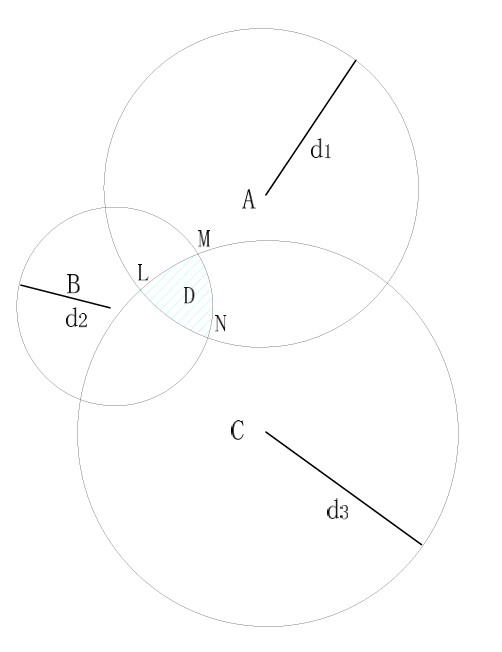
\includegraphics[width=0.5\linewidth]{img/fig2.jpg}
  \caption{Centroid positioning. D showing the possible positions of the robot, from beacon A, B, and C \cite{WSNCentroid}}
  \label{fig:centroid}
\end{figure}

We trained each model on the 1574-sample dataset (combining all distances) and reserved a held-out set of 236 real (non-synthetic) measurements for testing. During training, we optimized with a standard gradient-based optimizer (e.g.\ Adam) until convergence. For localization, each beacon’s predicted distance defines a circle around that beacon with radius equal to the estimated distance. We then apply the triangle‐centroid method: the unknown tag is located at the centroid of the intersection region of the three circles (Fig.~\ref{fig:centroid}). As Zhang and Zhao \cite{WSNCentroid} describe, the algorithm uses RSSI to measure distances $d$, treats the beacon node as the center of a circle, the distance $d$ as the radius of each circle, and obtains the unknown node location by seeking the centroid of the three-circle intersection. 

In practice we compute the pairwise intersection points of the circles and take their centroid as the position estimate. To reduce bias from larger errors at greater distances, we apply a distance-based weighting: intersections involving shorter predicted distances are given higher weight when computing the centroid. This follows the idea of weighted centroid localization \cite{nagah2021enhanced}. The final estimated coordinates are thus a weighted centroid of the three-circle intersection, which yields a single $(x,y)$ position. All steps above—from data collection through model training and localization—were implemented in TensorFlow and evaluated using the held-out test set of 236 samples. Performance was reported as the error between the true and estimated positions in the lab.

\begin{figure}[!b]
  \centering
  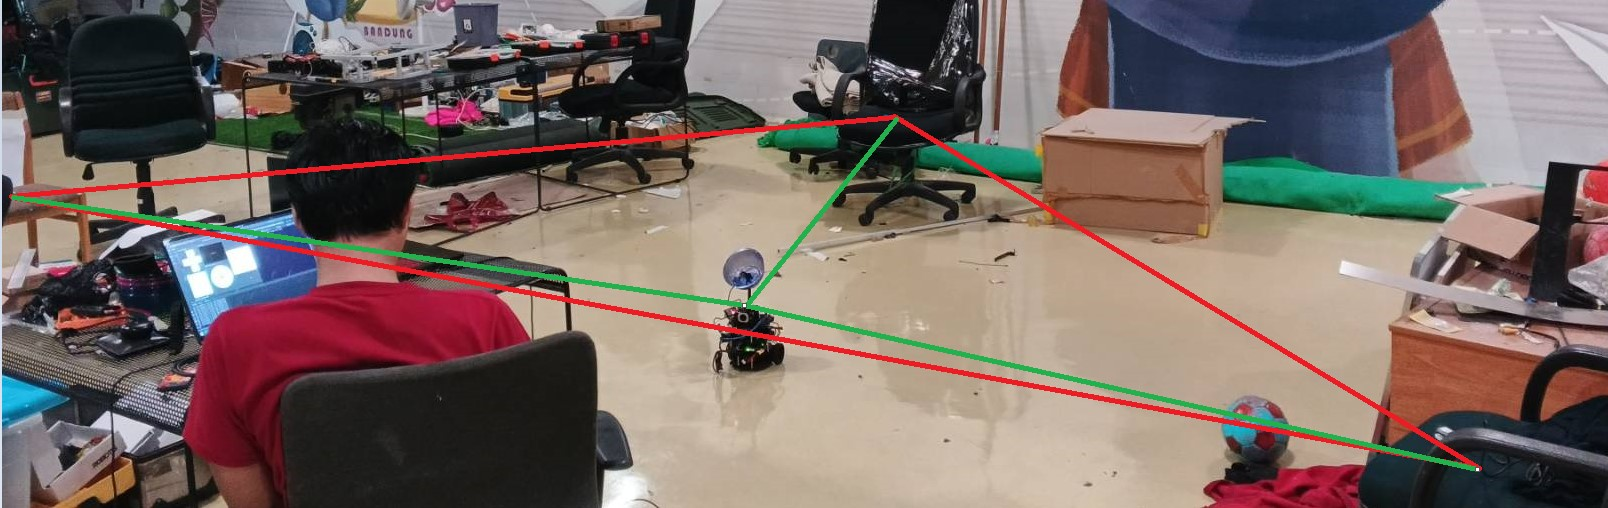
\includegraphics[width=0.75\linewidth]{img/rssi.jpg}
  \caption{Weighted Centroid Localization testing on different environment setup}
  \label{fig:environment}
\end{figure}

To evaluate generalization, we also performed \emph{cross-environment testing}: after training exclusively in the Labtek 1 environment, we deployed the same models and localization pipeline in a different indoor space as shown in Fig.~\ref{fig:environment}. RSSI data were collected at the same five distances under this new setting, and localization accuracy was measured without any retraining. This assessment demonstrates the robustness of our distance regression and weighted triangle-centroid method to changes in multipath and clutter.


\section{Results and Discussion}

\subsection{Voice Recognition Model Evaluation}
The proposed human voice detection model was evaluated on a held-out test set using multiple performance metrics, including accuracy, precision, recall, F1-score, and a confusion matrix. The test set comprised 3,622 audio clips, balanced across human and non-human classes.

The model achieved a final test accuracy of \textbf{97.79\%}, with a binary cross-entropy loss of 0.0909. The classification report is summarized in Table~\ref{tab:classification}.

\begin{table}[h]
\centering
\caption{Classification Performance on the Test Set}
\label{tab:classification}
\begin{tabular}{lcccc}
\toprule
\textbf{Class} & \textbf{Precision} & \textbf{Recall} & \textbf{F1-score} & \textbf{Support} \\
\midrule
Non-human (0) & 0.9723 & 0.9630 & 0.9676 & 1350 \\
Human (1)     & 0.9781 & 0.9837 & 0.9809 & 2272 \\
\midrule
\textbf{Accuracy} & \multicolumn{4}{c}{0.9760} \\
\textbf{Macro Avg} & 0.9752 & 0.9733 & 0.9743 & 3622 \\
\textbf{Weighted Avg} & 0.9760 & 0.9760 & 0.9760 & 3622 \\
\bottomrule
\end{tabular}
\end{table}

The confusion matrix in Table~\ref{tab:confusion} further illustrates the model’s performance:

\begin{table}[h]
\centering
\caption{Confusion Matrix}
\label{tab:confusion}
\begin{tabular}{ccc}
\toprule
 & \textbf{Predicted 0} & \textbf{Predicted 1} \\
\midrule
\textbf{Actual 0} & 1300 & 50 \\
\textbf{Actual 1} & 37 & 2235 \\
\bottomrule
\end{tabular}
\end{table}

The model shows strong recall for the human class (98.37\%), meaning it rarely misses vocal sounds in unseen test data—an important trait in SAR applications where false negatives (missed detections) are critical. The false positive rate is also low, indicating robustness against confusing non-human sounds.

These results confirm that a mel-spectrogram-based convolutional neural network, trained on real-world domestic sounds, can effectively distinguish human from non-human audio cues. The use of data augmentation techniques (e.g., time masking and additive noise) likely contributed to the model's generalization ability under variable acoustic conditions. Given its high accuracy and efficiency, this model is suitable for real-time deployment in embedded robotic platforms.

\section{Conclusion}
We have presented a modular, low-cost SAR robot framework combining TinyML audio detection with RSSI ranging. The platform’s hardware (ESP32 microcontrollers and simple sensors) and software (embedded neural network) are inherently cheap and power-efficient, aligning with the “low cost, simplicity, and commonly-available elements” desirable in SAR systems. 

The TinyML speech classifier proved highly effective, achieving ~97.8\% human-voice detection accuracy on the embedded device. This result is in line with recent work on microcontroller-based speech recognition, confirming that compact neural models can run reliably on battery-powered SAR robots. The RSSI-based localization method successfully provided approximate indoor positioning (mean error $\approx$0.5 m) without additional hardware. In practice, however, its accuracy is coarse and environment-dependent. As reported in prior studies, RSSI localization can suffer error variations due to walls, multipath, and interference. Our experiments reflected this: while the average error was sub-meter in open areas, it increased in cluttered or reflective spaces. Thus, the RSSI approach proved useful for rough triangulation but has clear limitations in precision.

Overall, our multi-modal SAR robot demonstrates that embedding intelligence in inexpensive hardware is viable for rescue scenarios. The combination of voice-based victim detection and wireless localization adds capability beyond basic tele-operation. In future deployments, such a system could be used to listen for survivors and guide responders even in NLOS conditions. In sum, the results show that a minimalist, sensor-rich design can offer real-world value, enabling a cost-effective SAR robot.

\section{Future Works}
\begin{itemize}
  \item \textbf{Improve RSSI Robustness:} Enhance the localization model to be more resilient to environmental factors. Possible approaches include dynamic calibration of the RSSI-distance model, machine-learning-based correction factors, or fusing RSSI with other signal features to reduce multipath error.
  \item \textbf{Multi-sensor Fusion:} Incorporate additional sensors (e.g. IMU, cameras, LIDAR) to strengthen situational awareness. Fusing inertial data and vision (e.g. depth or optical flow) with RSSI could significantly improve localization and mapping accuracy. For example, inertial measurements would help track the robot’s motion, and a camera could visually verify detected sound sources.
  \item \textbf{Dynamic Docking and Reconfiguration} Develop better physical interfaces and software for automated module coupling. Improving the robot’s ability to dock new modules (e.g. swapping or adding sensors) and reconfigure its shape would extend adaptability. Future designs might use spring-loaded connectors or magnetic alignment and implement software for hot-swapping modules on the fly.
  \item \textbf{Autonomous Navigation and Decision-Making} Integrate autonomous mobility and higher-level planning into the SAR robot. Future work should enable the robot to navigate indoor spaces (e.g. via SLAM algorithms), make path-planning decisions, and autonomously approach detected sound sources. In addition, machine-learning could be used for decision-making, such as prioritizing search areas or coordinating multiple robot units in a rescue mission.
\end{itemize}


\section{Ease of Use}

\subsection{Maintaining the Integrity of the Specifications}

The IEEEtran class file is used to format your paper and style the text. All margins, 
column widths, line spaces, and text fonts are prescribed; please do not 
alter them. You may note peculiarities. For example, the head margin
measures proportionately more than is customary. This measurement 
and others are deliberate, using specifications that anticipate your paper 
as one part of the entire proceedings, and not as an independent document. 
Please do not revise any of the current designations.

\section{Prepare Your Paper Before Styling}
Before you begin to format your paper, first write and save the content as a 
separate text file. Complete all content and organizational editing before 
formatting. Please note sections \ref{AA}--\ref{SCM} below for more information on 
proofreading, spelling and grammar.

Keep your text and graphic files separate until after the text has been 
formatted and styled. Do not number text heads---{\LaTeX} will do that 
for you.

\subsection{Abbreviations and Acronyms}\label{AA}
Define abbreviations and acronyms the first time they are used in the text, 
even after they have been defined in the abstract. Abbreviations such as 
IEEE, SI, MKS, CGS, ac, dc, and rms do not have to be defined. Do not use 
abbreviations in the title or heads unless they are unavoidable.

\subsection{Units}
\begin{itemize}
\item Use either SI (MKS) or CGS as primary units. (SI units are encouraged.) English units may be used as secondary units (in parentheses). An exception would be the use of English units as identifiers in trade, such as ``3.5-inch disk drive''.
\item Avoid combining SI and CGS units, such as current in amperes and magnetic field in oersteds. This often leads to confusion because equations do not balance dimensionally. If you must use mixed units, clearly state the units for each quantity that you use in an equation.
\item Do not mix complete spellings and abbreviations of units: ``Wb/m\textsuperscript{2}'' or ``webers per square meter'', not ``webers/m\textsuperscript{2}''. Spell out units when they appear in text: ``. . . a few henries'', not ``. . . a few H''.
\item Use a zero before decimal points: ``0.25'', not ``.25''. Use ``cm\textsuperscript{3}'', not ``cc''.)
\end{itemize}

\subsection{Equations}
Number equations consecutively. To make your 
equations more compact, you may use the solidus (~/~), the exp function, or 
appropriate exponents. Italicize Roman symbols for quantities and variables, 
but not Greek symbols. Use a long dash rather than a hyphen for a minus 
sign. Punctuate equations with commas or periods when they are part of a 
sentence, as in:
\begin{equation}
a+b=\gamma\label{eq}
\end{equation}

Be sure that the 
symbols in your equation have been defined before or immediately following 
the equation. Use ``\eqref{eq}'', not ``Eq.~\eqref{eq}'' or ``equation \eqref{eq}'', except at 
the beginning of a sentence: ``Equation \eqref{eq} is . . .''

\subsection{\LaTeX-Specific Advice}

Please use ``soft'' (e.g., \verb|\eqref{Eq}|) cross references instead
of ``hard'' references (e.g., \verb|(1)|). That will make it possible
to combine sections, add equations, or change the order of figures or
citations without having to go through the file line by line.

Please don't use the \verb|{eqnarray}| equation environment. Use
\verb|{align}| or \verb|{IEEEeqnarray}| instead. The \verb|{eqnarray}|
environment leaves unsightly spaces around relation symbols.

Please note that the \verb|{subequations}| environment in {\LaTeX}
will increment the main equation counter even when there are no
equation numbers displayed. If you forget that, you might write an
article in which the equation numbers skip from (17) to (20), causing
the copy editors to wonder if you've discovered a new method of
counting.

{\BibTeX} does not work by magic. It doesn't get the bibliographic
data from thin air but from .bib files. If you use {\BibTeX} to produce a
bibliography you must send the .bib files. 

{\LaTeX} can't read your mind. If you assign the same label to a
subsubsection and a table, you might find that Table I has been cross
referenced as Table IV-B3. 

{\LaTeX} does not have precognitive abilities. If you put a
\verb|\label| command before the command that updates the counter it's
supposed to be using, the label will pick up the last counter to be
cross referenced instead. In particular, a \verb|\label| command
should not go before the caption of a figure or a table.

Do not use \verb|\nonumber| inside the \verb|{array}| environment. It
will not stop equation numbers inside \verb|{array}| (there won't be
any anyway) and it might stop a wanted equation number in the
surrounding equation.

\subsection{Some Common Mistakes}\label{SCM}
\begin{itemize}
\item The word ``data'' is plural, not singular.
\item The subscript for the permeability of vacuum $\mu_{0}$, and other common scientific constants, is zero with subscript formatting, not a lowercase letter ``o''.
\item In American English, commas, semicolons, periods, question and exclamation marks are located within quotation marks only when a complete thought or name is cited, such as a title or full quotation. When quotation marks are used, instead of a bold or italic typeface, to highlight a word or phrase, punctuation should appear outside of the quotation marks. A parenthetical phrase or statement at the end of a sentence is punctuated outside of the closing parenthesis (like this). (A parenthetical sentence is punctuated within the parentheses.)
\item A graph within a graph is an ``inset'', not an ``insert''. The word alternatively is preferred to the word ``alternately'' (unless you really mean something that alternates).
\item Do not use the word ``essentially'' to mean ``approximately'' or ``effectively''.
\item In your paper title, if the words ``that uses'' can accurately replace the word ``using'', capitalize the ``u''; if not, keep using lower-cased.
\item Be aware of the different meanings of the homophones ``affect'' and ``effect'', ``complement'' and ``compliment'', ``discreet'' and ``discrete'', ``principal'' and ``principle''.
\item Do not confuse ``imply'' and ``infer''.
\item The prefix ``non'' is not a word; it should be joined to the word it modifies, usually without a hyphen.
\item There is no period after the ``et'' in the Latin abbreviation ``et al.''.
\item The abbreviation ``i.e.'' means ``that is'', and the abbreviation ``e.g.'' means ``for example''.
\end{itemize}
An excellent style manual for science writers is \cite{b7}.

\subsection{Authors and Affiliations}
\textbf{The class file is designed for, but not limited to, six authors.} A 
minimum of one author is required for all conference articles. Author names 
should be listed starting from left to right and then moving down to the 
next line. This is the author sequence that will be used in future citations 
and by indexing services. Names should not be listed in columns nor group by 
affiliation. Please keep your affiliations as succinct as possible (for 
example, do not differentiate among departments of the same organization).

\subsection{Identify the Headings}
Headings, or heads, are organizational devices that guide the reader through 
your paper. There are two types: component heads and text heads.

Component heads identify the different components of your paper and are not 
topically subordinate to each other. Examples include Acknowledgments and 
References and, for these, the correct style to use is ``Heading 5''. Use 
``figure caption'' for your Figure captions, and ``table head'' for your 
table title. Run-in heads, such as ``Abstract'', will require you to apply a 
style (in this case, italic) in addition to the style provided by the drop 
down menu to differentiate the head from the text.

Text heads organize the topics on a relational, hierarchical basis. For 
example, the paper title is the primary text head because all subsequent 
material relates and elaborates on this one topic. If there are two or more 
sub-topics, the next level head (uppercase Roman numerals) should be used 
and, conversely, if there are not at least two sub-topics, then no subheads 
should be introduced.

\subsection{Figures and Tables}
\paragraph{Positioning Figures and Tables} Place figures and tables at the top and 
bottom of columns. Avoid placing them in the middle of columns. Large 
figures and tables may span across both columns. Figure captions should be 
below the figures; table heads should appear above the tables. Insert 
figures and tables after they are cited in the text. Use the abbreviation 
``Fig.~\ref{fig}'', even at the beginning of a sentence.

\begin{table}[htbp]
\caption{Table Type Styles}
\begin{center}
\begin{tabular}{|c|c|c|c|}
\hline
\textbf{Table}&\multicolumn{3}{|c|}{\textbf{Table Column Head}} \\
\cline{2-4} 
\textbf{Head} & \textbf{\textit{Table column subhead}}& \textbf{\textit{Subhead}}& \textbf{\textit{Subhead}} \\
\hline
copy& More table copy$^{\mathrm{a}}$& &  \\
\hline
\multicolumn{4}{l}{$^{\mathrm{a}}$Sample of a Table footnote.}
\end{tabular}
\label{tab1}
\end{center}
\end{table}

\begin{figure}[htbp]
\centerline{
\includegraphics{fig1.png}}
\caption{Example of a figure caption.}
\label{fig}
\end{figure}

Figure Labels: Use 8 point Times New Roman for Figure labels. Use words 
rather than symbols or abbreviations when writing Figure axis labels to 
avoid confusing the reader. As an example, write the quantity 
``Magnetization'', or ``Magnetization, M'', not just ``M''. If including 
units in the label, present them within parentheses. Do not label axes only 
with units. In the example, write ``Magnetization (A/m)'' or ``Magnetization 
\{A[m(1)]\}'', not just ``A/m''. Do not label axes with a ratio of 
quantities and units. For example, write ``Temperature (K)'', not 
``Temperature/K''.

% \section*{Acknowledgment}

% The preferred spelling of the word ``acknowledgment'' in America is without 
% an ``e'' after the ``g''. Avoid the stilted expression ``one of us (R. B. 
% G.) thanks $\ldots$''. Instead, try ``R. B. G. thanks$\ldots$''. Put sponsor 
% acknowledgments in the unnumbered footnote on the first page.

% \section*{References}

% Please number citations consecutively within brackets \cite{b1}. The 
% sentence punctuation follows the bracket \cite{b2}. Refer simply to the reference 
% number, as in \cite{b3}---do not use ``Ref. \cite{b3}'' or ``reference \cite{b3}'' except at 
% the beginning of a sentence: ``Reference \cite{b3} was the first $\ldots$''

% Number footnotes separately in superscripts. Place the actual footnote at 
% the bottom of the column in which it was cited. Do not put footnotes in the 
% abstract or reference list. Use letters for table footnotes.

% Unless there are six authors or more give all authors' names; do not use 
% ``et al.''. Papers that have not been published, even if they have been 
% submitted for publication, should be cited as ``unpublished'' \cite{b4}. Papers 
% that have been accepted for publication should be cited as ``in press'' \cite{b5}. 
% Capitalize only the first word in a paper title, except for proper nouns and 
% element symbols.

% For papers published in translation journals, please give the English 
% citation first, followed by the original foreign-language citation \cite{b6}.

\begingroup
\raggedright
\bibliographystyle{IEEEtran}
\bibliography{references}
\endgroup

% \begin{thebibliography}{00}
% \bibitem{b1} G. Eason, B. Noble, and I. N. Sneddon, ``On certain integrals of Lipschitz-Hankel type involving products of Bessel functions,'' Phil. Trans. Roy. Soc. London, vol. A247, pp. 529--551, April 1955.
% \bibitem{b2} J. Clerk Maxwell, A Treatise on Electricity and Magnetism, 3rd ed., vol. 2. Oxford: Clarendon, 1892, pp.68--73.
% \bibitem{b3} I. S. Jacobs and C. P. Bean, ``Fine particles, thin films and exchange anisotropy,'' in Magnetism, vol. III, G. T. Rado and H. Suhl, Eds. New York: Academic, 1963, pp. 271--350.
% \bibitem{b4} K. Elissa, ``Title of paper if known,'' unpublished.
% \bibitem{b5} R. Nicole, ``Title of paper with only first word capitalized,'' J. Name Stand. Abbrev., in press.
% \bibitem{b6} Y. Yorozu, M. Hirano, K. Oka, and Y. Tagawa, ``Electron spectroscopy studies on magneto-optical media and plastic substrate interface,'' IEEE Transl. J. Magn. Japan, vol. 2, pp. 740--741, August 1987 [Digests 9th Annual Conf. Magnetics Japan, p. 301, 1982].
% \bibitem{b7} M. Young, The Technical Writer's Handbook. Mill Valley, CA: University Science, 1989.
% \end{thebibliography}
% \vspace{12pt}
% \color{red}
% IEEE conference templates contain guidance text for composing and formatting conference papers. Please ensure that all template text is removed from your conference paper prior to submission to the conference. Failure to remove the template text from your paper may result in your paper not being published.

\end{document}
